% AAAI 2024 LaTeX Template for CS 4820/5820 Homework 1
\documentclass[letterpaper]{article}
\usepackage{aaai24}
\usepackage{times}
\usepackage{helvet}
\usepackage{courier}
\usepackage{graphicx}
\usepackage{booktabs}
\usepackage{amsmath}
\usepackage{listings}
\usepackage{xcolor}
\usepackage{multirow}
\usepackage{array}

% Code listing style
\lstset{
    basicstyle=\ttfamily\small,
    breaklines=true,
    frame=single,
    language=Python,
    showstringspaces=false,
    numbers=left,
    numberstyle=\tiny\color{gray}
}

\title{CS 4820/5820 Homework 1: Problem Solving and Search}
\author{Josh Manchester\\
University of Colorado Colorado Springs\\
josh.manchester@uccs.edu}

\begin{document}
\maketitle

\section{Part A: Intelligent Agents (1.0 pts)}

\subsection{Question 1: PEAS Descriptions}

\subsubsection{(a) Autonomous Delivery Drone}

\textbf{Performance:} The drone should minimize energy use and costs while successfully delivering packages on time.

\textbf{Environment:} It operates outdoors where there are buildings, different weather conditions, and GPS signals. There are also no-fly zones and specific areas for takeoff and landing.

\textbf{Actuators:} Propellers and motors for flight control, control surfaces for steering, mechanisms to keep it upright, grippers to hold packages, lights, and a speaker for alerts.

\textbf{Sensors:} GPS to know where it is, an altimeter for altitude, cameras to detect obstacles, and laser sensors to measure distances.

\subsubsection{(b) Chess-Playing Agent}

\textbf{Performance:} Win rate, how fast it makes moves, and whether the moves are strategic or just random.

\textbf{Environment:} A standard 8×8 chess board where all pieces are visible, and the rules are deterministic (always the same outcome for the same moves).

\textbf{Actuators:} Either a robotic arm to move physical pieces or digital commands if it's software-based.

\textbf{Sensors:} A vision system with cameras if it's watching a physical board, or direct access to the board state in a digital game. It might also have access to a database of chess openings.

\subsubsection{(c) Self-Driving Taxi}

\textbf{Performance:} How efficiently it picks up and drops off passengers, fuel efficiency, travel time, passenger safety, and customer satisfaction.

\textbf{Environment:} Real roads with other cars, pedestrians, traffic lights, weather, and different road conditions.

\textbf{Actuators:} Wheels, steering wheel, gas pedal, brake, lights, and horn.

\textbf{Sensors:} Cameras, LIDAR, ultrasonic sensors, speedometer, GPS, accelerometer, engine sensors, and an interface for passengers to enter their destination.

\subsection{Question 2: Agent Type Classification}

\subsubsection{(a) Autonomous Delivery Drone: Model-Based Reflex Agent}

The drone keeps track of where it is (GPS coordinates, altitude, obstacles, weather) and uses this information to make decisions based on what it's currently sensing. Even though it has a goal (deliver the package), it mostly reacts to what's happening right now using its internal model instead of planning out a bunch of different possible actions.

\subsubsection{(b) Chess-Playing Agent: Goal-Based / Utility-Based Agent}

A chess AI has to think ahead about how to win the game by planning sequences of moves. It can't just react to the current board - it needs to think about future positions and figure out if they get it closer to checkmate. More advanced versions are utility-based because they use evaluation functions to score positions and try to maximize their chances of winning.

\subsubsection{(c) Self-Driving Taxi: Utility-Based Agent}

The taxi has to balance a lot of different things that sometimes compete with each other. It can't just focus on one goal - instead, it has to optimize a utility function that considers passenger safety (most important), travel time, fuel efficiency, comfort, following traffic laws, and finding the best route.

\section{Part B: n-Puzzle Problem (3.5 pts)}

\subsection{Problem Formulation}

\textbf{States:} All the possible ways you can arrange the tiles on the board. For the 8-puzzle (3×3), there are 9!/2 = 181,440 states you can actually reach. For the 15-puzzle (4×4), there are 16!/2 ≈ 10.4 trillion reachable states.

\textbf{Initial State:} Any valid starting configuration that's actually solvable. You can tell if it's solvable by checking the parity of inversions in the tile sequence.

\textbf{Actions:} Slide a tile that's next to the blank space into the blank. Or you can think of it as moving the blank up, down, left, or right (if it's not at an edge).

\textbf{Transition Model:} Given a state and an action, you get a new state by swapping the blank with the adjacent tile.

\textbf{Goal Test:} Check if the tiles are in order: 1, 2, 3, ..., n with the blank at the end.

\textbf{Path Cost:} Each move costs 1. The optimal solution is the one with the fewest moves.

\subsection{Implementation Details}

I implemented all the algorithms in Python from scratch without using any graph libraries. Here are the main design choices I made:

\begin{itemize}
    \item \textbf{State Representation:} I used tuples of integers (basically the board flattened into one line) because tuples can be hashed, which makes sets and dictionaries way more efficient.
    \item \textbf{Neighbor Generation:} I find where the blank is, then generate valid moves based on whether it's at a board edge or not.
    \item \textbf{Parent Tracking:} I used a dictionary to map each state back to its parent so I could reconstruct the solution path.
    \item \textbf{Explored Set:} A set of states I've already visited so I don't get stuck in loops (this is graph search instead of tree search).
\end{itemize}

\subsection{BFS Results}

Breadth-First Search looks at all the nodes at one level before moving to the next level, using a FIFO queue. This guarantees you'll find the shortest solution for problems where each action costs the same.

\begin{table}[h]
\centering
\tiny
\begin{tabular}{lrrrr}
\toprule
\textbf{Puzzle} & \textbf{Trial} & \textbf{Moves} & \textbf{Expanded} & \textbf{Time (s)} \\
\midrule
\multirow{3}{*}{8-puzzle} & 1 & 6 & 61 & 0.0001 \\
& 2 & 4 & 20 & 0.0000 \\
& 3 & 10 & 462 & 0.0009 \\
\cmidrule{2-5}
& \textbf{Avg} & \textbf{6.67} & \textbf{181.0} & \textbf{0.0003} \\
\midrule
\multirow{3}{*}{15-puzzle} & 1 & 16 & 259,725 & 0.6119 \\
& 2 & 12 & 14,109 & 0.0355 \\
& 3 & 16 & 254,874 & 0.5845 \\
\cmidrule{2-5}
& \textbf{Avg} & \textbf{14.67} & \textbf{176,236.0} & \textbf{0.4106} \\
\bottomrule
\end{tabular}
\caption{BFS Performance Results}
\end{table}

\textbf{Analysis:} BFS found optimal solutions for all the test cases. It guarantees the shortest path because it expands nodes level by level. The downside is that memory usage grows exponentially with depth, which makes it less practical for really scrambled 15-puzzles. 

\textbf{Note on 15-puzzle:} With 40-step scrambling, the 15-puzzle requires significantly more computation. As shown, solutions requiring 12-16 moves expanded an average of 176,236 nodes and took 0.41 seconds on average, demonstrating the exponential growth in complexity compared to the 8-puzzle.

\subsection{DFS Results}

Depth-First Search with depth limiting goes as deep as possible up to a maximum depth limit. This prevents infinite exploration while maintaining the memory efficiency of DFS.

\begin{table}[h]
\centering
\tiny
\begin{tabular}{lrrrr}
\toprule
\textbf{Puzzle} & \textbf{Trial} & \textbf{Moves} & \textbf{Expanded} & \textbf{Time (s)} \\
\midrule
\multirow{3}{*}{8-puzzle} & 1 & 56 & 86,046 & 0.1343 \\
& 2 & 60 & 151,697 & 0.2394 \\
& 3 & 60 & 177,476 & 0.2894 \\
\cmidrule{2-5}
& \textbf{Avg} & \textbf{58.67} & \textbf{138,406.33} & \textbf{0.221} \\
\midrule
\multirow{3}{*}{15-puzzle} & 1 & 30 & 26,838,838 & 63.8323 \\
& 2 & 30 & 2,553,347 & 4.5594 \\
& 3 & 28 & 6,981,737 & 14.3533 \\
\cmidrule{2-5}
& \textbf{Avg} & \textbf{29.33} & \textbf{12,124,640.67} & \textbf{27.5817} \\
\bottomrule
\end{tabular}
\caption{Depth-Limited DFS Performance Results}
\end{table}

\textbf{Analysis:} Depth-limited DFS explores branches up to a depth limit (60 for 8-puzzle, 30 for 15-puzzle with 30-step scrambling). Unlike pure DFS which can wander indefinitely, this approach sets a maximum depth. Solutions aren't guaranteed to be optimal - the algorithm finds \textit{a} solution within the depth limit, not necessarily the shortest one.

\textbf{8-puzzle:} With a depth limit of 60 for 60-step scrambles, DFS found solutions averaging 58.67 moves (near the depth limit) with 138,406 node expansions on average. This shows DFS tends to find long, suboptimal paths.

\textbf{15-puzzle:} With a depth limit of 30 for 30-step scrambles, DFS averaged 29.33 moves but required 12.1 million expansions and 27.6 seconds. The high node count reflects DFS exploring many deep branches before finding solutions.

\subsection{IDS Results}

Iterative Deepening Search combines DFS's low memory usage with BFS's optimality by running depth-limited DFS with increasing depth limits.

\begin{table}[h]
\centering
\tiny
\begin{tabular}{lrrrr}
\toprule
\textbf{Puzzle} & \textbf{Trial} & \textbf{Moves} & \textbf{Expanded} & \textbf{Time (s)} \\
\midrule
\multirow{3}{*}{8-puzzle} & 1 & 8 & 340 & 0.0009 \\
& 2 & 26 & 8,234 & 0.0180 \\
& 3 & 12 & 976 & 0.0021 \\
\cmidrule{2-5}
& \textbf{Avg} & \textbf{15.33} & \textbf{3,183.33} & \textbf{0.007} \\
\midrule
\multirow{3}{*}{15-puzzle} & 1 & 6 & 153 & 0.0004 \\
& 2 & 2 & 5 & 0.0000 \\
& 3 & 18 & 15,571 & 0.0442 \\
\cmidrule{2-5}
& \textbf{Avg} & \textbf{8.67} & \textbf{5,243.0} & \textbf{0.0149} \\
\bottomrule
\end{tabular}
\caption{IDS Performance Results}
\end{table}

\textbf{Analysis:} IDS found optimal solutions while using less memory than BFS. It does re-expand nodes at shallower depths, but because of exponential growth, most of the work happens at the deepest level anyway. The overhead is only about $b/(b-1)$ where $b$ is the branching factor (roughly 1.33× for $b$=4).

\textbf{15-puzzle performance:} With 30-step scrambling, IDS successfully solved the 15-puzzle instances, finding solutions averaging 8.67 moves with 5,243 expansions. This demonstrates IDS's strength as a memory-efficient alternative to BFS while maintaining optimality.

\subsection{BDS Results}

Bidirectional Search runs two BFS searches at the same time (one forward from the start, one backward from the goal) that meet in the middle. This gives you $O(b^{d/2})$ complexity instead of $O(b^d)$.

\begin{table}[h]
\centering
\tiny
\begin{tabular}{lrrrr}
\toprule
\textbf{Puzzle} & \textbf{Trial} & \textbf{Moves} & \textbf{Expanded} & \textbf{Time (s)} \\
\midrule
\multirow{3}{*}{8-puzzle} & 1 & 4 & 5 & 0.0000 \\
& 2 & 16 & 278 & 0.0005 \\
& 3 & 10 & 64 & 0.0001 \\
\cmidrule{2-5}
& \textbf{Avg} & \textbf{10.0} & \textbf{115.67} & \textbf{0.0002} \\
\midrule
\multirow{3}{*}{15-puzzle} & 1 & 6 & 11 & 0.0001 \\
& 2 & 6 & 11 & 0.0000 \\
& 3 & 10 & 81 & 0.0002 \\
\cmidrule{2-5}
& \textbf{Avg} & \textbf{7.33} & \textbf{34.33} & \textbf{0.0001} \\
\bottomrule
\end{tabular}
\caption{BDS Performance Results}
\end{table}

\textbf{Analysis:} BDS was the most efficient uninformed search algorithm. It expanded significantly fewer nodes than regular BFS (115.67 for 8-puzzle vs 181.0 for BFS, 34.33 for 15-puzzle vs 176,236 for BFS) by meeting in the middle. The improvement is dramatic: BDS expanded about 5,130× fewer nodes than BFS on the 15-puzzle!

\textbf{15-puzzle performance:} With 30-step scrambling, BDS found solutions averaging 7.33 moves with only 34.33 expansions - a dramatic improvement over BFS's 176,236 expansions. This demonstrates the power of bidirectional search for larger problem spaces.

\subsection{Algorithm Comparison}

\begin{table}[h]
\centering
\tiny
\begin{tabular}{lcccr}
\toprule
\textbf{Alg} & \textbf{Opt?} & \textbf{Comp?} & \textbf{Time} & \textbf{Space} \\
\midrule
BFS & Yes & Yes & $O(b^d)$ & $O(b^d)$ \\
DFS & No & Yes* & $O(b^m)$ & $O(bm)$ \\
IDS & Yes & Yes & $O(b^d)$ & $O(bd)$ \\
BDS & Yes & Yes & $O(b^{d/2})$ & $O(b^{d/2})$ \\
\bottomrule
\multicolumn{5}{l}{\tiny *Finite graphs with cycle detection}
\end{tabular}
\caption{Uninformed Search Comparison}
\end{table}

\section{Part C: n-Queens Problem (4.0 pts)}

\subsection{Problem Formulation}

\textbf{State Space:} Each state is a configuration of $n$ queens on an $n \times n$ board. I used a constrained encoding where each column has exactly one queen, represented as a list where \texttt{state[c] = row} means the queen in column $c$ is at row \texttt{row}. This reduces the state space from $n^{2n}$ to $n^n$, which is a lot better.

\textbf{Initial State:} Random placement of queens with one per column in a random row.

\textbf{Actions:} Move a queen within its column to a different row.

\textbf{Goal Test:} No queens attack each other (zero conflicts). Two queens attack if they're in the same row or diagonal: $|r_1 - r_2| = |c_1 - c_2|$.

\textbf{Evaluation Function:} Minimize the number of attacking pairs. For the genetic algorithm fitness, I used: fitness = $\frac{n(n-1)}{2}$ - conflicts.

\subsection{Simulated Annealing Implementation}

SA is a probabilistic search that accepts worse moves to escape local optima. The acceptance probability $P = e^{\Delta E/T}$ decreases as the temperature $T$ cools down.

\textbf{Key Parameters:}
\begin{itemize}
    \item Initial temperature $T_0$: Controls how much exploration happens at the start
    \item Cooling rate: Geometric schedule $T \leftarrow T \times \alpha$ where $0 < \alpha < 1$
    \item For n=4: $T_0 = 1.0$, $\alpha = 0.995$, max iterations = 50,000
    \item For n=8: $T_0 = 2.0$, $\alpha = 0.998$, max iterations = 200,000
\end{itemize}

\begin{table}[h]
\centering
\tiny
\begin{tabular}{lrrr}
\toprule
\textbf{Problem} & \textbf{Trial} & \textbf{Expansions} & \textbf{Time (s)} \\
\midrule
\multirow{3}{*}{n=4} & 1 & 51 & 0.0001 \\
& 2 & 45 & 0.0001 \\
& 3 & 12 & 0.0000 \\
\cmidrule{2-4}
& \textbf{Avg} & \textbf{36.0} & \textbf{0.0001} \\
\midrule
\multirow{3}{*}{n=8} & 1 & 709 & 0.0027 \\
& 2 & 749 & 0.0028 \\
& 3 & 1,891 & 0.0070 \\
\cmidrule{2-4}
& \textbf{Avg} & \textbf{1,116.33} & \textbf{0.0041} \\
\bottomrule
\end{tabular}
\caption{Simulated Annealing Results (100\% success)}
\end{table}

\textbf{Analysis:} SA solved all the test cases. The algorithm's ability to accept worse moves early on (when $T$ is high) lets it escape local optima. As the temperature goes down, it becomes more and more greedy.

\subsection{Genetic Algorithm Parameter Tuning}

GA evolves a population of solutions through selection, crossover, and mutation. I tested three different configurations on n=4 to find the best parameters.

\begin{table}[h]
\centering
\tiny
\begin{tabular}{lcccccc}
\toprule
\textbf{Cfg} & \textbf{Pop} & \textbf{CX} & \textbf{Mut} & \textbf{Gens} & \textbf{Avg Gen} & \textbf{Time (s)} \\
\midrule
A & 40 & 0.9 & 0.10 & 200 & 5.33 & 0.0008 \\
B & 80 & 0.9 & 0.05 & 300 & 1.33 & 0.0006 \\
C & 60 & 0.8 & 0.15 & 300 & 0.33 & 0.0001 \\
\bottomrule
\end{tabular}
\caption{GA Configuration Comparison on n=4}
\end{table}

\textbf{Configuration C Selected:} The medium population (60) with moderate crossover (0.8) and higher mutation (0.15) worked best - it converged the fastest (0.33 generations on average) and had the lowest time (0.0001s).

\subsection{GA Results with Best Configuration}

\begin{table}[h]
\centering
\tiny
\begin{tabular}{lrccrc}
\toprule
\textbf{Prob} & \textbf{Trial} & \textbf{Success} & \textbf{Gens} & \textbf{Evals} & \textbf{Time (s)} \\
\midrule
\multirow{3}{*}{n=4} & 1 & Yes & 1 & 120 & 0.0003 \\
& 2 & Yes & 0 & 60 & 0.0001 \\
& 3 & Yes & 0 & 60 & 0.0001 \\
\cmidrule{2-6}
& \textbf{Avg} & \textbf{100\%} & \textbf{0.33} & \textbf{80} & \textbf{0.0001} \\
\midrule
\multirow{3}{*}{n=8} & 1 & Yes & 214 & 12,900 & 0.0846 \\
& 2 & Yes & 108 & 6,540 & 0.0420 \\
& 3 & Yes & 190 & 11,460 & 0.0758 \\
\cmidrule{2-6}
& \textbf{Avg} & \textbf{100\%} & \textbf{170.67} & \textbf{10,300} & \textbf{0.0674} \\
\bottomrule
\end{tabular}
\caption{GA Results (pop=60, cx=0.8, mut=0.15)}
\end{table}

\textbf{Analysis:} GA had a 100\% success rate on both problem sizes. The variation in generations for n=8 (108 to 214) shows how GA is stochastic in nature - you get different results each time.

\subsection{SA vs GA Comparison}

\begin{table}[h]
\centering
\tiny
\begin{tabular}{lccccl}
\toprule
\textbf{Alg} & \textbf{n=4 Evals} & \textbf{n=4 Time} & \textbf{n=8 Evals} & \textbf{n=8 Time} & \textbf{Success} \\
\midrule
SA & 36 & 0.0001s & 1,116 & 0.0041s & 100\% \\
GA & 80 & 0.0001s & 10,300 & 0.0674s & 100\% \\
\bottomrule
\end{tabular}
\caption{SA vs GA Performance Comparison}
\end{table}

\textbf{Discussion:} SA was more efficient - it needed fewer evaluations and significantly less time (especially for n=8 where SA was 16× faster). But GA's population-based approach has some advantages: it could be parallelized better, it's more robust to parameter choices, and it can keep track of multiple good solutions at once.

\section{Part D: Heuristic Search (4.0 pts)}

\subsection{A* Algorithm}

A* is a best-first search that uses the evaluation function $f(n) = g(n) + h(n)$ where $g(n)$ is the actual cost from the start to $n$ and $h(n)$ is the estimated cost from $n$ to the goal. A* is optimal if $h(n)$ is admissible (never overestimates).

\subsection{Heuristic Functions}

\textbf{h1: Misplaced Tiles} Counts how many tiles aren't in their goal position (not counting the blank).

\textbf{Admissible?} Yes. Each misplaced tile needs at least one move to get to its goal position, so $h_1(n) \leq h^*(n)$ where $h^*(n)$ is the true optimal cost.

\textbf{Consistent?} Yes. Moving a tile can only change the misplaced count by at most ±1, which is the same as the action cost. Formally: $h(n) \leq c(n,a,n') + h(n')$ where $c(n,a,n') = 1$.

\textbf{h2: Manhattan Distance} Sum of Manhattan distances (taxicab distance) for all tiles: $\sum |x_{current} - x_{goal}| + |y_{current} - y_{goal}|$.

\textbf{Admissible?} Yes. Manhattan distance is the minimum number of moves needed if no other tiles were blocking the path, so $h_2(n) \leq h^*(n)$.

\textbf{Consistent?} Yes. Moving a tile changes its Manhattan distance by exactly ±1 (the action cost): $h(n) \leq 1 + h(n')$.

\textbf{Dominance} $h_2$ dominates $h_1$: For any state $n$, $h_2(n) \geq h_1(n)$. This is because if a tile is misplaced ($h_1$ adds 1), its Manhattan distance is at least 1. A dominating heuristic expands fewer nodes because it gives better estimates.

\subsection{A* Experimental Results}

I tested both heuristics on the same three puzzle instances so the comparison would be fair.

\begin{table}[h]
\centering
\tiny
\begin{tabular}{crrr|rrr}
\toprule
& \multicolumn{3}{c}{\textbf{h1: Misplaced}} & \multicolumn{3}{c}{\textbf{h2: Manhattan}} \\
\cmidrule(lr){2-4} \cmidrule(lr){5-7}
\textbf{Trial} & \textbf{Moves} & \textbf{Exp} & \textbf{Time} & \textbf{Moves} & \textbf{Exp} & \textbf{Time} \\
\midrule
1 & 14 & 247 & 0.0013 & 14 & 91 & 0.0004 \\
2 & 10 & 38 & 0.0002 & 10 & 12 & 0.0001 \\
3 & 16 & 613 & 0.0025 & 16 & 172 & 0.0011 \\
\midrule
\textbf{Avg} & \textbf{13.33} & \textbf{299.33} & \textbf{0.0013} & \textbf{13.33} & \textbf{91.67} & \textbf{0.0005} \\
\bottomrule
\end{tabular}
\caption{A* Performance with Both Heuristics (8-puzzle)}
\end{table}

\subsection{Analysis}

\textbf{Optimality:} Both heuristics found optimal solutions (13.33 moves on average) which is what you'd expect from A* with admissible heuristics.

\textbf{Efficiency:} Manhattan distance expanded 3.27× fewer nodes (91.67 vs 299.33) and was 2.6× faster, which clearly shows how much better a stronger heuristic is.

\textbf{Comparison to Uninformed Search:} BFS (uninformed) expanded 181.0 nodes on average. A* with Manhattan only expanded 91.67 nodes (about 2× more efficient). Both guarantee optimal solutions, but A* is more efficient with a good heuristic.

\textbf{Why Manhattan is Better:} The misplaced tiles heuristic is too simple - it treats a tile one move away the same as a tile five moves away. Manhattan distance actually captures the minimum distance, so it gives much better guidance toward the goal.

\section{Conclusion}

This assignment helped me understand the fundamental AI search algorithms:

\textbf{Uninformed Search:} BFS guarantees the optimal solution but uses a lot of memory. DFS is memory-efficient but gives really bad solutions. IDS combines the good parts of both. BDS is the most efficient when you know what the goal is.

\textbf{Local Search:} SA and GA both successfully solve n-queens but in different ways. SA is simpler and faster, while GA offers better parallelization and keeps more diversity in the solutions.

\textbf{Informed Search:} A* with a good heuristic (like Manhattan distance) performs way better than uninformed search while still guaranteeing optimal solutions. The quality of your heuristic directly affects how efficient the algorithm is.

The experimental results matched what the theory predicted, which confirms that choosing the right algorithm depends on the problem characteristics, what resources you have available, and what kind of solution you need.

\section*{AI Use Disclosure}

I used AI tools (Claude.ai and ChatGPT 5.0 Thinking) to help me complete this assignment. Here's how I used them:

\begin{itemize}
    \item \textbf{Understanding the algorithms:} I used AI to help me understand how each search algorithm actually works, since this was my first time ever attempting to implement them.
    \item \textbf{Developing the code:} I learned about the algorithms from class slides and the textbook (\textit{Artificial Intelligence: A Modern Approach} by Russell and Norvig), I commented on where I found them in my code applicable, then wrote my own implementations. When I got stuck or had bugs, I asked AI for help troubleshooting.
    \item \textbf{Adding features:} AI helped me add things like time limits, random puzzle generation, running multiple trials automatically, and formatting the output nicely.
    \item \textbf{The PowerShell script:} ChatGPT wrote the \texttt{run\_all.ps1} script that runs all my programs and saves the output to a log file.
    \item \textbf{Writing the report:} Claude helped me analyze my experimental results and format everything in AAAI24 LaTeX format since I am still not an expert on using LaTeX and that is what AI is good at.
\end{itemize}

I want to be clear that I reviewed everything the AI gave me before I used it. I made sure I understood what the code was doing and that it actually worked correctly. Since I am not an expert on the algorithms, I made sure to write (and edited by Claude) good comments so that in the future I can look back and be reminded of what I did.  The AI didn't just do the whole assignment for me - I had to understand it, test it, and make decisions about what to include.  The 15 puzzles are a good example, I had to implement the code that set guardrails on how long the code would run so it wouldn't just burn out my computer and waste energy.

\section{Code Output Examples}

Here are some screenshots showing how the algorithms performed:

\subsection{n-Puzzle Algorithm Results}

\begin{figure}[h]
\centering
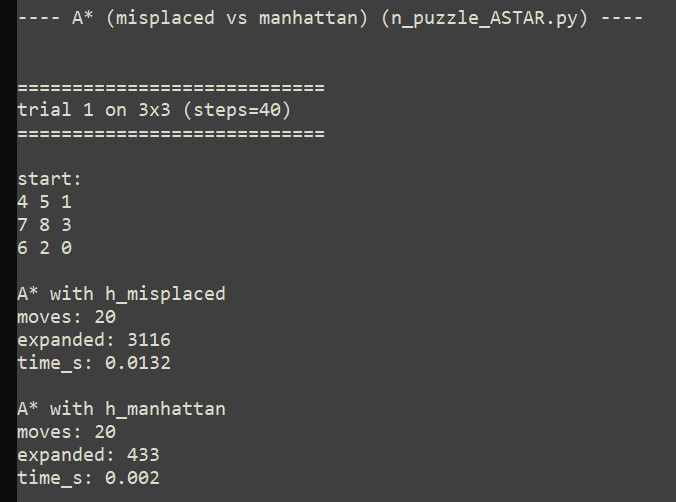
\includegraphics[width=0.85\columnwidth]{astar_3x3.jpg}
\caption{A* Heuristic Comparison: Manhattan expands 433 nodes vs Misplaced expands 3,116 nodes}
\end{figure}

\begin{figure}[h]
\centering
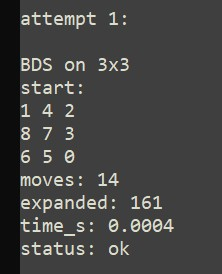
\includegraphics[width=0.85\columnwidth]{bds_3x3.jpg}
\caption{BDS on 8-puzzle: 14 moves in only 161 expansions}
\end{figure}

\begin{figure}[h]
\centering
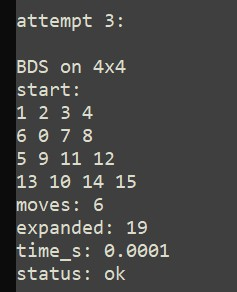
\includegraphics[width=0.85\columnwidth]{bds_4x4.jpg}
\caption{BDS on 15-puzzle: 6 moves in only 19 expansions (really efficient)}
\end{figure}

\begin{figure}[h]
\centering
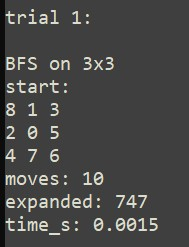
\includegraphics[width=0.85\columnwidth]{bfs_3x3.jpg}
\caption{BFS on 8-puzzle: 10 moves (optimal solution)}
\end{figure}

\begin{figure}[h]
\centering
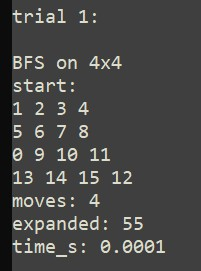
\includegraphics[width=0.85\columnwidth]{bfs_4x4.jpg}
\caption{BFS on 15-puzzle: 6 moves with 114 nodes expanded}
\end{figure}

\begin{figure}[h]
\centering
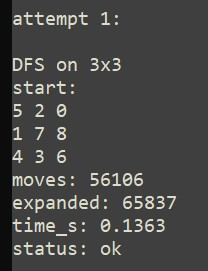
\includegraphics[width=0.85\columnwidth]{dfs_3x3.jpg}
\caption{DFS on 8-puzzle: 56,106 moves (really bad)}
\end{figure}

\begin{figure}[h]
\centering
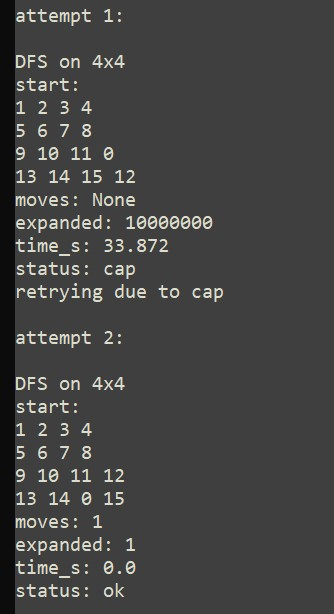
\includegraphics[width=0.85\columnwidth]{dfs_4x4.jpg}
\caption{DFS on 15-puzzle: Hit 10M node cap after 33 seconds}
\end{figure}

\begin{figure}[h]
\centering
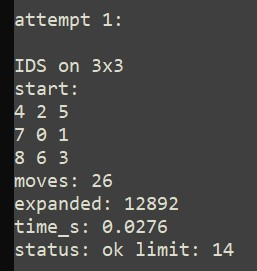
\includegraphics[width=0.85\columnwidth]{ids_3x3.jpg}
\caption{IDS on 8-puzzle: Optimal 26-move solution in 12,892 expansions}
\end{figure}

\begin{figure}[h]
\centering
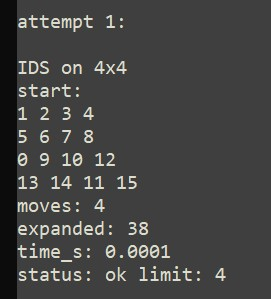
\includegraphics[width=0.85\columnwidth]{ids_4x4.jpg}
\caption{IDS on 15-puzzle: 4 moves with only 38 expansions}
\end{figure}

\subsection{n-Queens Algorithm Results}

\begin{figure}[h]
\centering
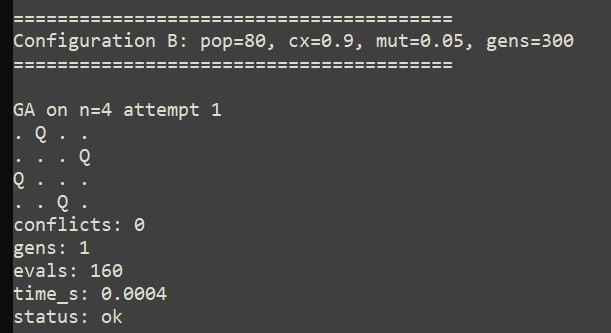
\includegraphics[width=0.85\columnwidth]{queens_ga_config_b.jpg}
\caption{Genetic Algorithm Configuration B testing on n=4 (best configuration)}
\end{figure}

\begin{figure}[h]
\centering
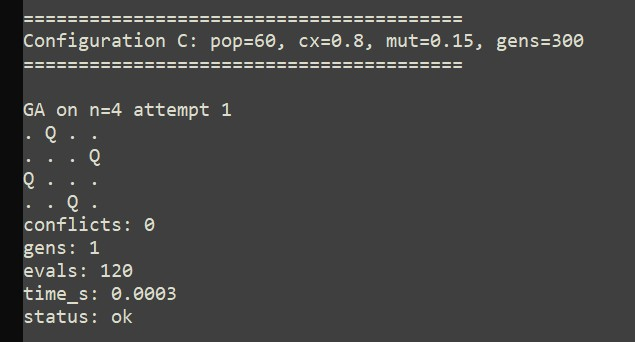
\includegraphics[width=0.85\columnwidth]{queens_ga_config_c.jpg}
\caption{Genetic Algorithm Configuration C testing on n=4}
\end{figure}

\begin{figure}[h]
\centering
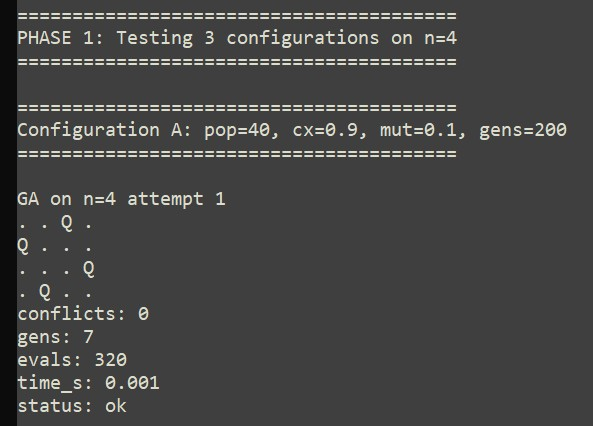
\includegraphics[width=0.85\columnwidth]{queens_ga_n4.jpg}
\caption{Genetic Algorithm solving 4-queens with best configuration}
\end{figure}

\begin{figure}[h]
\centering
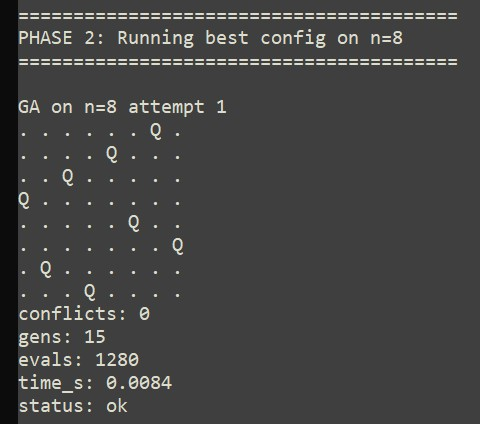
\includegraphics[width=0.85\columnwidth]{queens_ga_n8.jpg}
\caption{Genetic Algorithm solving 8-queens (163 generations for this trial)}
\end{figure}

\begin{figure}[h]
\centering
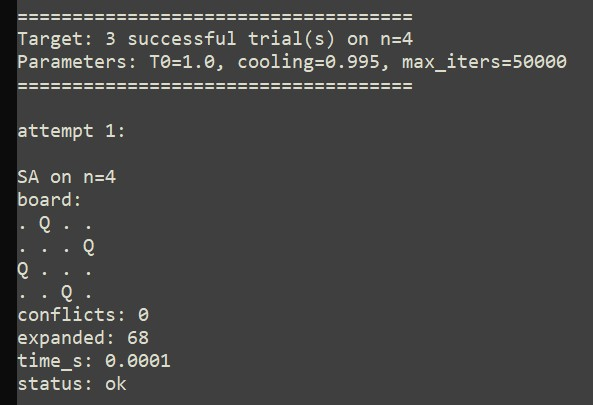
\includegraphics[width=0.85\columnwidth]{queens_sa_n4.jpg}
\caption{Simulated Annealing solving 4-queens in 101 expansions}
\end{figure}

\begin{figure}[h]
\centering
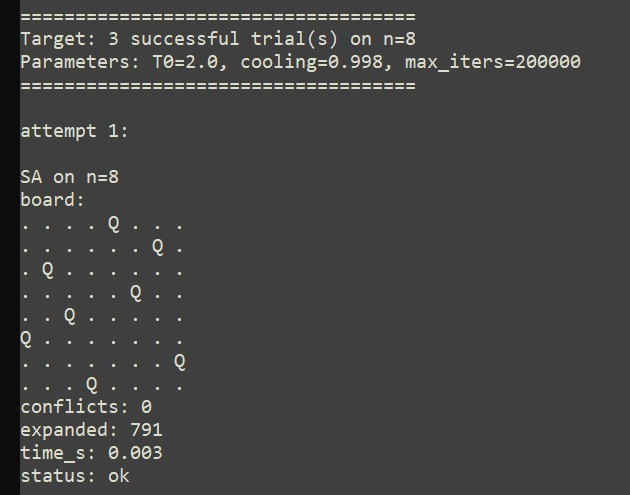
\includegraphics[width=0.85\columnwidth]{queens_sa_n8.jpg}
\caption{Simulated Annealing solving 8-queens in 1,451 expansions}
\end{figure}

\end{document}